\pagebreak
\newpage

\pagebreak
\newpage

\section{Classifier}

Classifiers were developed for three cases.

\begin{itemize}
 \item Classifier with $\Sigma = \sigma^2 \cdot \mathbf{I}$
 \item Classifier with $\Sigma = \Sigma_i$
 \item Classifier with arbitrary $\Sigma$
\end{itemize}


\subsection{Case A}
For the first case, $\sigma$ was assigned as $\sigma = 0.25$.
Given this restriction, the multivariate PDF was obtained, as shown in Figure \ref{fig: case a PDF}

\begin{figure}[htb!]
\centering
 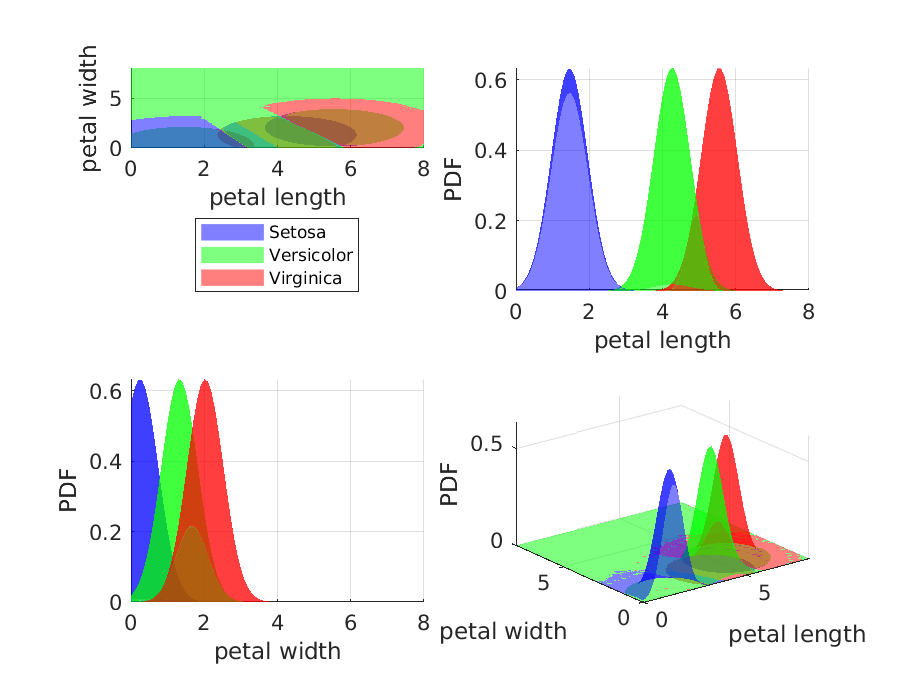
\includegraphics[width = 0.8\textwidth]{pdfCaseA}
 \caption{PDF for Case A}
 \label{fig: case a PDF}
\end{figure}

\begin{align*}
 g_i(x) &= - \frac{\norm{x-\mu_i}^2}{2\sigma^2} + \ln P(\omega_i)\\
 \norm{x-\mu_i}^2 &= (x-\mu_i)^T (x-\mu_i)\\
 g_i(x) &= w^T_i x + \omega_{i0}\\
 w_i &= \frac{1}{\sigma^2} \mu\\
 w_{i0} &= \frac{-1}{2 \sigma^2} \mu^T_i \mu_i + ļn P(\omega_i)
\end{align*}


\pagebreak
\newpage


Afterwards, the \emph{a posteriori} probability is obtained and the boundaries of the classifier are obtained.
The results are shown in Figure \ref{fig: posteriori case A}.

\begin{figure}[htb!]
\centering
 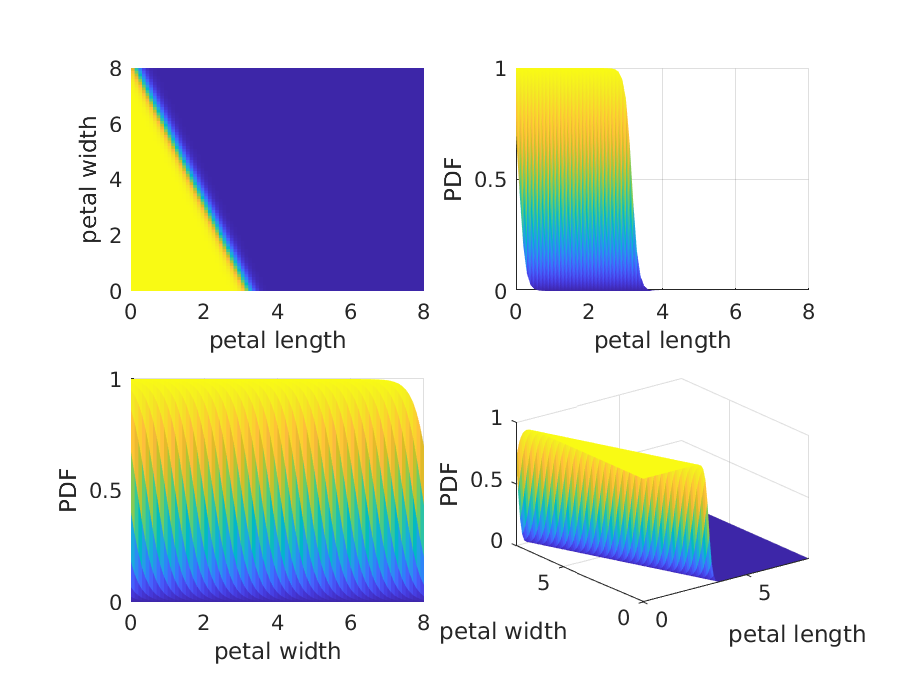
\includegraphics[width= 0.8\textwidth]{classifierSetosaCaseA}
 \caption{Case A - A posteriori probability}
 \label{fig: posteriori case A}
\end{figure}




\pagebreak
\newpage


The classifier was tested against a sample of 75 entries from the dataset. Each entry was assigned a colour based on the assigned variety:
yellow for Setosa, black for Versicolor and magenta for Virginica.
This is presented in Figure \ref{fig: classifier case A}.

\begin{figure}[htb!]
\centering
 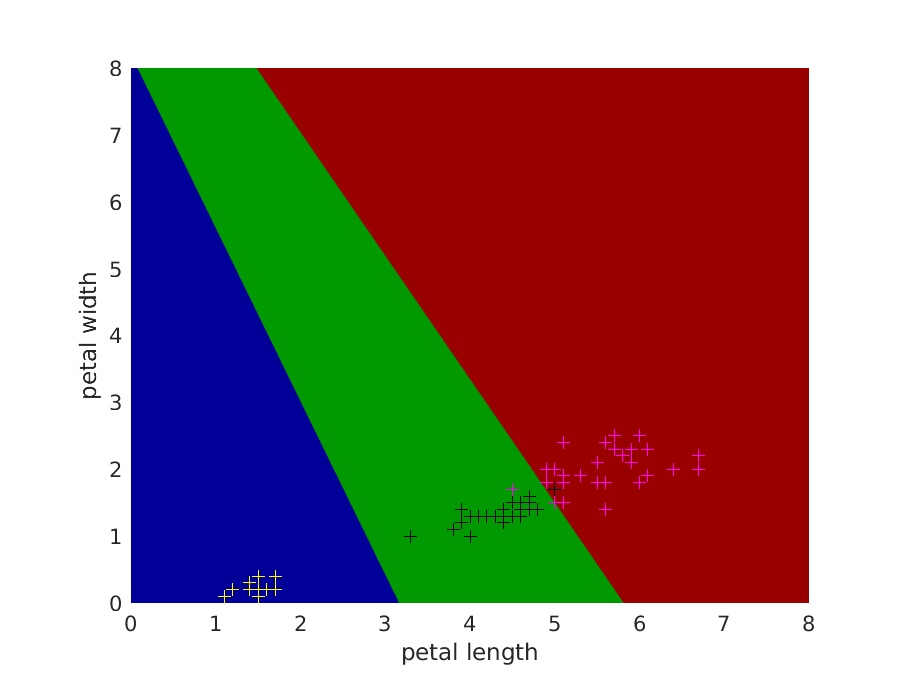
\includegraphics[width= \textwidth]{testClassifierCaseA}
 \caption{Case A - Boundaries}
 \label{fig: classifier case A}
\end{figure}




\pagebreak
\newpage

\pagebreak
\newpage

\subsection{Case B}
For the first case, $\Sigma$ was assigned as

\begin{equation*}
 \begin{pmatrix}
  0.26 & 0.04 &  0.02 & 0.01 \\
  0.04 &  0.22 & 0.03 & 0.02 \\
  0.02 & 0.03 & 0.15 & 0.15\\
  0.01 & 0.02 &  0.15 & 0.31
 \end{pmatrix}
\end{equation*}

This new covariance matrix influenced the multivariate gaussian distribution of the system,
as seen in Figure \ref{fig: case b PDF}.

\begin{figure}[htb!]
 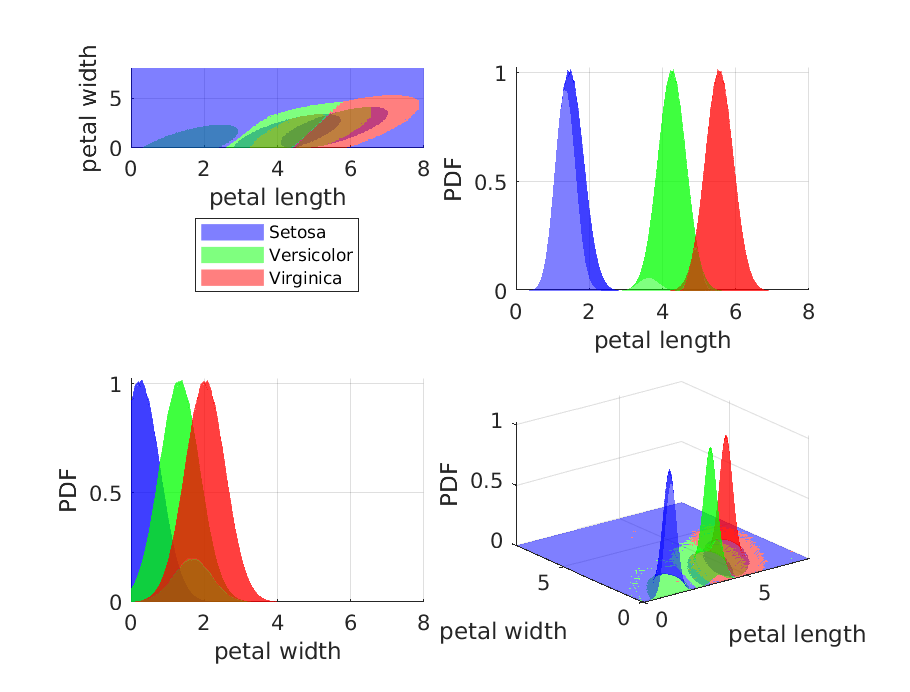
\includegraphics[width = \textwidth]{pdfCaseB}
 \caption{PDF for Case B}
 \label{fig: case b PDF}
\end{figure}

\pagebreak
\newpage


Afterwards, the \emph{a posteriori} probability is obtained and the boundaries of the classifier are obtained.
The results are shown in Figure \ref{fig: posteriori case B}.

\begin{figure}[htb!]
\centering
 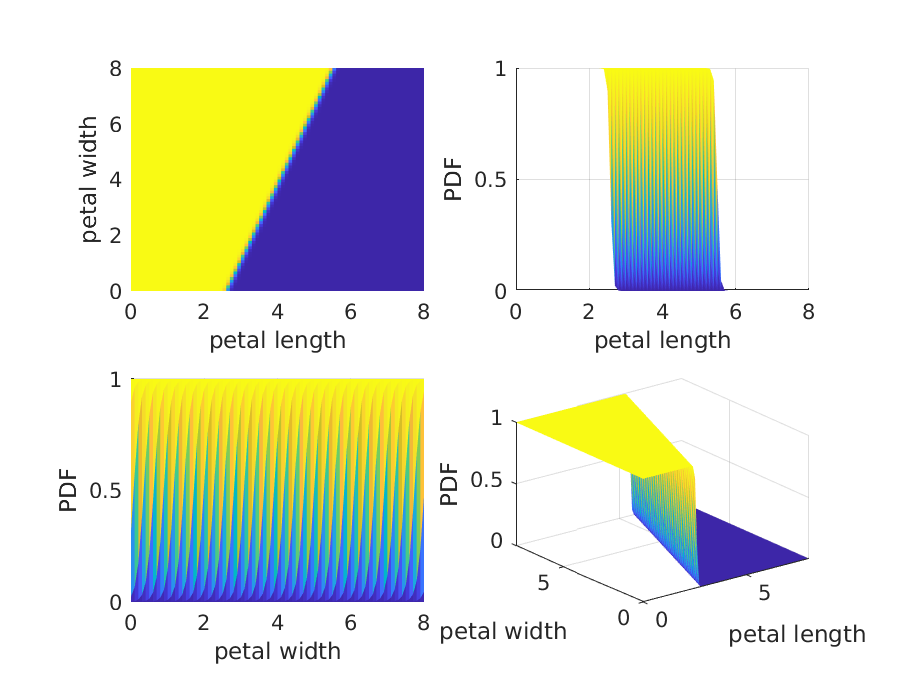
\includegraphics[width= 0.8\textwidth]{classifierSetosaCaseB}
 \caption{Case B - A posteriori probability}
 \label{fig: posteriori case B}
\end{figure}

\begin{align*}
 g_i(x) &= x^T W_i x + w^T_i x + \omega_{i0}\\
 W_i &= -\frac{1}{2}\Sigma^{-1}_i\\
 w_i &= \Sigma^{-1}_i \mu_i\\
 \omega_{i0}&= -\frac{1}{2} \mu^T_i \Sigma^{-1}_i \mu_i - \frac{1}{2}\ln \det(\Sigma_i) + \ln P(\omega_i)
\end{align*}

\pagebreak
\newpage


The classifier was tested against a sample of 75 entries from the dataset. Each entry was assigned a colour based on the assigned variety:
yellow for Setosa, black for Versicolor and magenta for Virginica.
This is presented in Figure \ref{fig: classifier case B}.

\begin{figure}[htb!]
\centering
 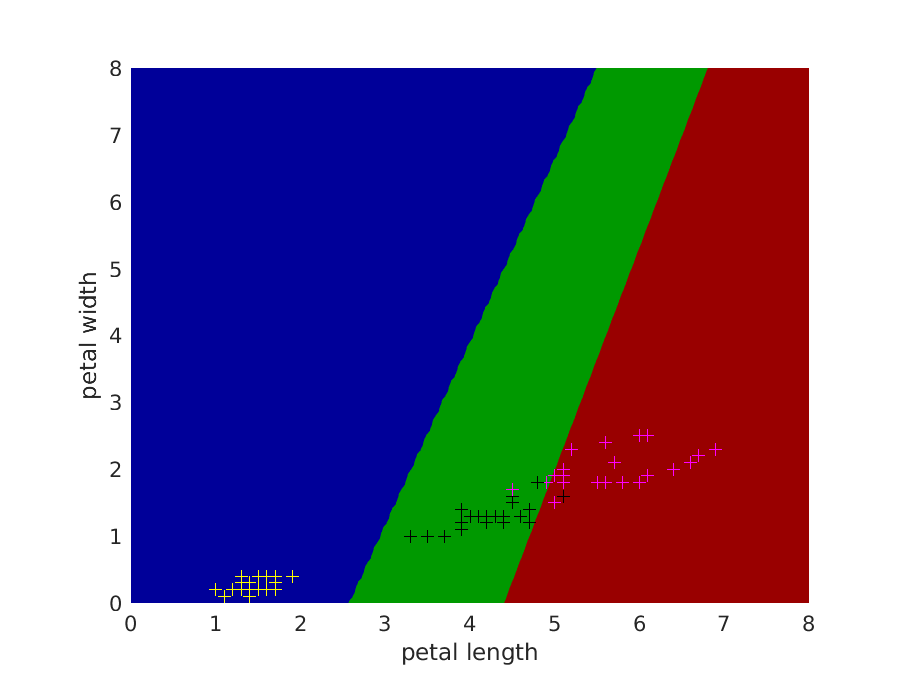
\includegraphics[width= \textwidth]{testClassifierCaseB}
 \caption{Case B - Boundaries}
 \label{fig: classifier case B}
\end{figure}

\pagebreak
\newpage


\pagebreak
\newpage

\subsection{Case C}
For the third case, $\Sigma$ was left untouched, allowing the covariance matrix to
reflect the nature of the data available.
This is observed in Figure \ref{fig: case c PDF}.

\begin{figure}[htb!]
 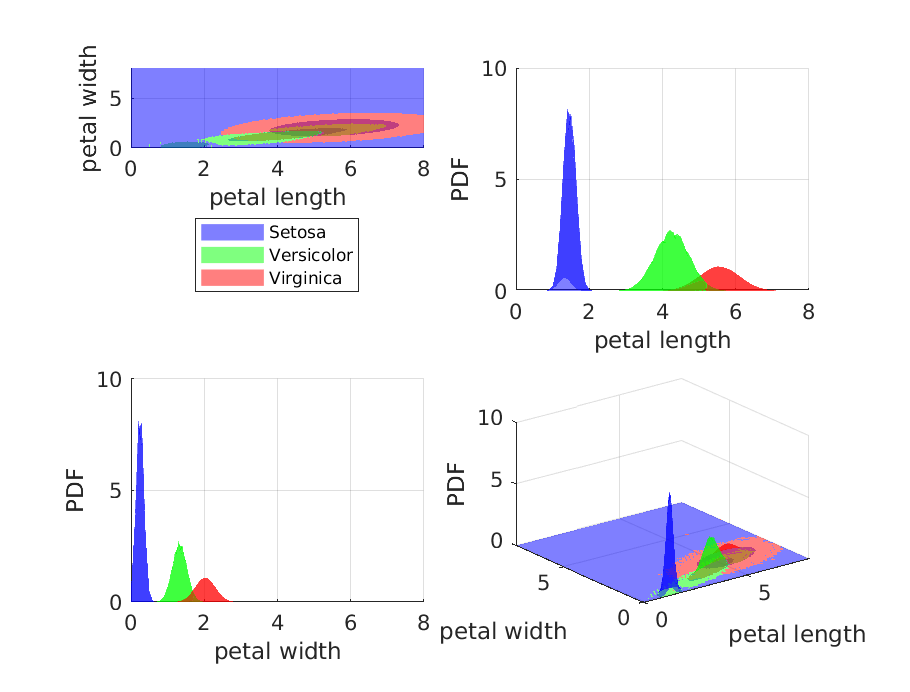
\includegraphics[width = \textwidth]{pdfCaseC}
 \caption{PDF for Case C}
 \label{fig: case c PDF}
\end{figure}

\pagebreak
\newpage


Afterwards, the \emph{a posteriori} probability is obtained and the boundaries of the classifier are obtained.
The results are shown in Figure \ref{fig: posteriori case C}.

\begin{figure}[htb!]
\centering
 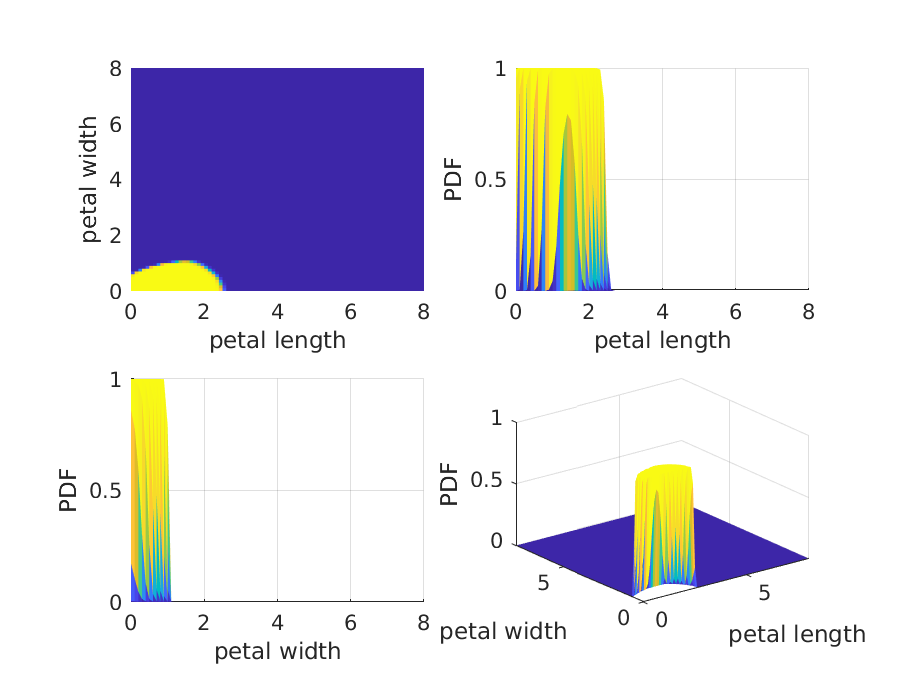
\includegraphics[width= 0.8\textwidth]{classifierSetosaCaseC}
 \caption{Case C - A posteriori probability}
 \label{fig: posteriori case C}
\end{figure}

\pagebreak
\newpage

\begin{align*}
 g_i(x) &= -\frac{1}{2} (x-\mu_i)^T \Sigma^{-1} (x-\mu) + \ln P(\omega_i)\\
 g_i(x) &= w^T_i x + \omega_{i0}\\
 w_i &= \Sigma^{-1} \mu_i\\
 w_{i0} &= \frac{-1}{2}\mu^T_i \Sigma^{-1}  \mu_i + ļn P(\omega_i)
\end{align*}

The classifier was tested against a sample of 75 entries from the dataset. Each entry was assigned a colour based on the assigned variety:
yellow for Setosa, black for Versicolor and magenta for Virginica.
This is presented in Figure \ref{fig: classifier case C}.

\begin{figure}[htb!]
\centering
 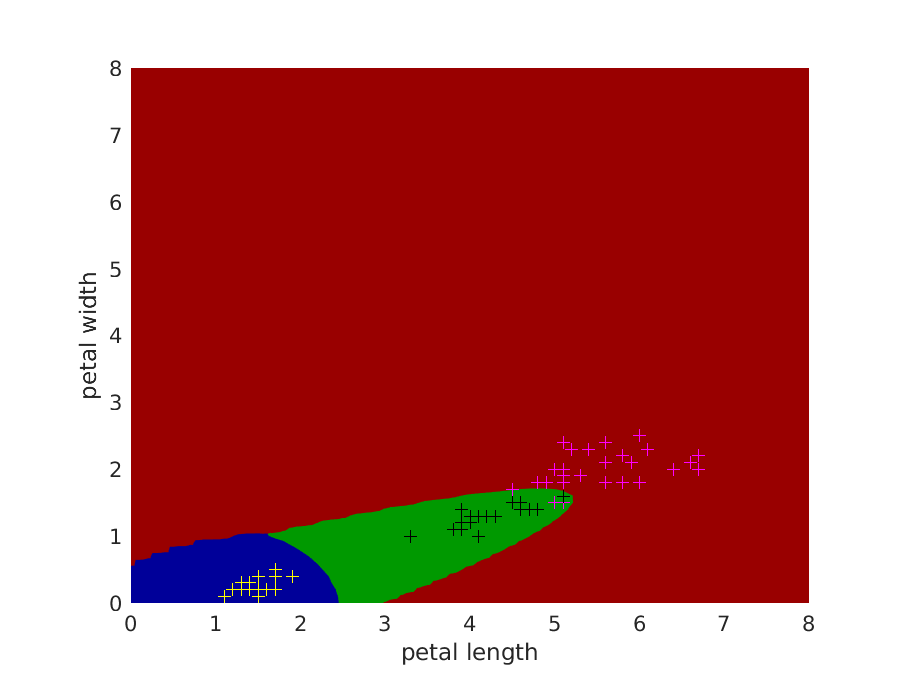
\includegraphics[width= \textwidth]{testClassifierCaseC}
 \caption{Case C - Boundaries}
 \label{fig: classifier case C}
\end{figure}

\pagebreak
\newpage
